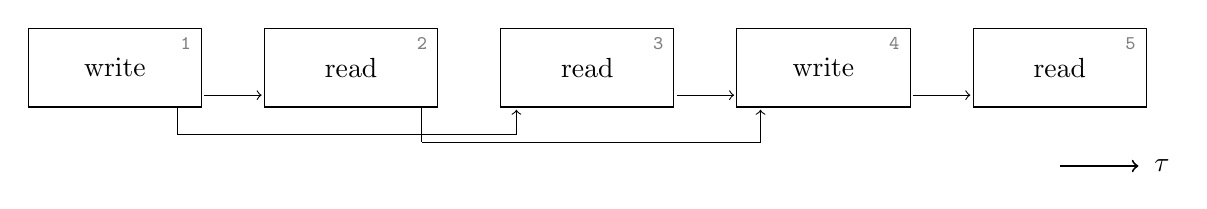
\begin{tikzpicture}
    \node[style=draw, minimum width=2.2cm, minimum height=1cm] at (0, -0.25) {write};
    \node[style=draw, minimum width=2.2cm, minimum height=1cm] at (3, -0.25) {read};
    \node[style=draw, minimum width=2.2cm, minimum height=1cm] at (6, -0.25) {read};
    \node[style=draw, minimum width=2.2cm, minimum height=1cm] at (9, -0.25) {write};
    \node[style=draw, minimum width=2.2cm, minimum height=1cm] at (12, -0.25) {read};

    \node[gray, font=\scriptsize] at (0.9, 0.05) {\texttt{1}};
    \node[gray, font=\scriptsize] at (3.9, 0.05) {\texttt{2}};
    \node[gray, font=\scriptsize] at (6.9, 0.05) {\texttt{3}};
    \node[gray, font=\scriptsize] at (9.9, 0.05) {\texttt{4}};
    \node[gray, font=\scriptsize] at (12.9, 0.05) {\texttt{5}};

    % 0-1
    \draw[->, shorten >=1pt, shorten <=1pt] (1.1,-0.6) -- (1.9,-0.6);

    % 2-3
    \draw[->, shorten >=1pt, shorten <=1pt] (7.1,-0.6) -- (7.9,-0.6);

    % 3-4
    \draw[->, shorten >=1pt, shorten <=1pt] (10.1,-0.6) -- (10.9,-0.6);

    % 0-2
    \draw (0.8,-0.75) -- (0.8,-1.1);
    \draw (0.8,-1.1) -- (5.1,-1.1);
    \draw[->, shorten >=1pt] (5.1,-1.1) -- (5.1,-0.75);

    % 1-3
    \draw (3.9,-0.75) -- (3.9,-1.2);
    \draw (3.9,-1.2) -- (8.2,-1.2);
    \draw[->, shorten >=1pt] (8.2,-1.2) -- (8.2,-0.75);

    \node[font=\itshape] (time) at (13.3, -1.5) {$\tau$};
    \draw[line width=0.7pt, ->] (12, -1.5) to (13, -1.5);
\end{tikzpicture}